\section{Streudiagramme}\label{sec:scatterplots}
Die nachfolgende \autoref{table:correlations-overview} zeigt die jeweiligen Korrelationen zwischen Hypothesen mit einem Korrelationskoeffizienten ohne Anwendung der Funktion \texttt{jitter}. Aufgrund dessen, dass der p-Wert unter dem festgelegten Signifikanzniveau $\alpha$ von $0,05$ liegt, sind die vorliegenden Korrelationen alle statistisch signifikant. 

\begin{table}[ht]
\centering
\begin{tabular}{ c | c | c | c}
  Relation & Spearmans $\rho$ & p-Wert & signifikant?\\
  \hline
  \hline
  H1 - H11 & $0,52$ & $1,1e-06$ & \cmark \\
  H1 - H12 & $0,54$ & $2,4e-07$ & \cmark \\
  H2 - H3 & $0,55$ & $1,5e-07$ & \cmark \\
  H11 - H12 & $0,76$ & $4,2e-16$ & \cmark \\
  H13 - H14 & $0,72$ & $9,5e-14$ & \cmark
\end{tabular}
\caption{Korrelationen zwischen Hypothesen im Überblick}
\label{table:correlations-overview}
\end{table}

Alle nachfolgenden Abbildungen zeigen Streudiagramme nach Anwendung der Funktion \texttt{jitter}. Diese wurde verwendet, um Werte voneinander unterscheiden zu können. Es sei angemerkt, dass dies R- und p-Werte verfälscht und die korrekten Werte in \autoref{table:correlations-overview} zu sehen sind.

\begin{figure}[H]
\centering
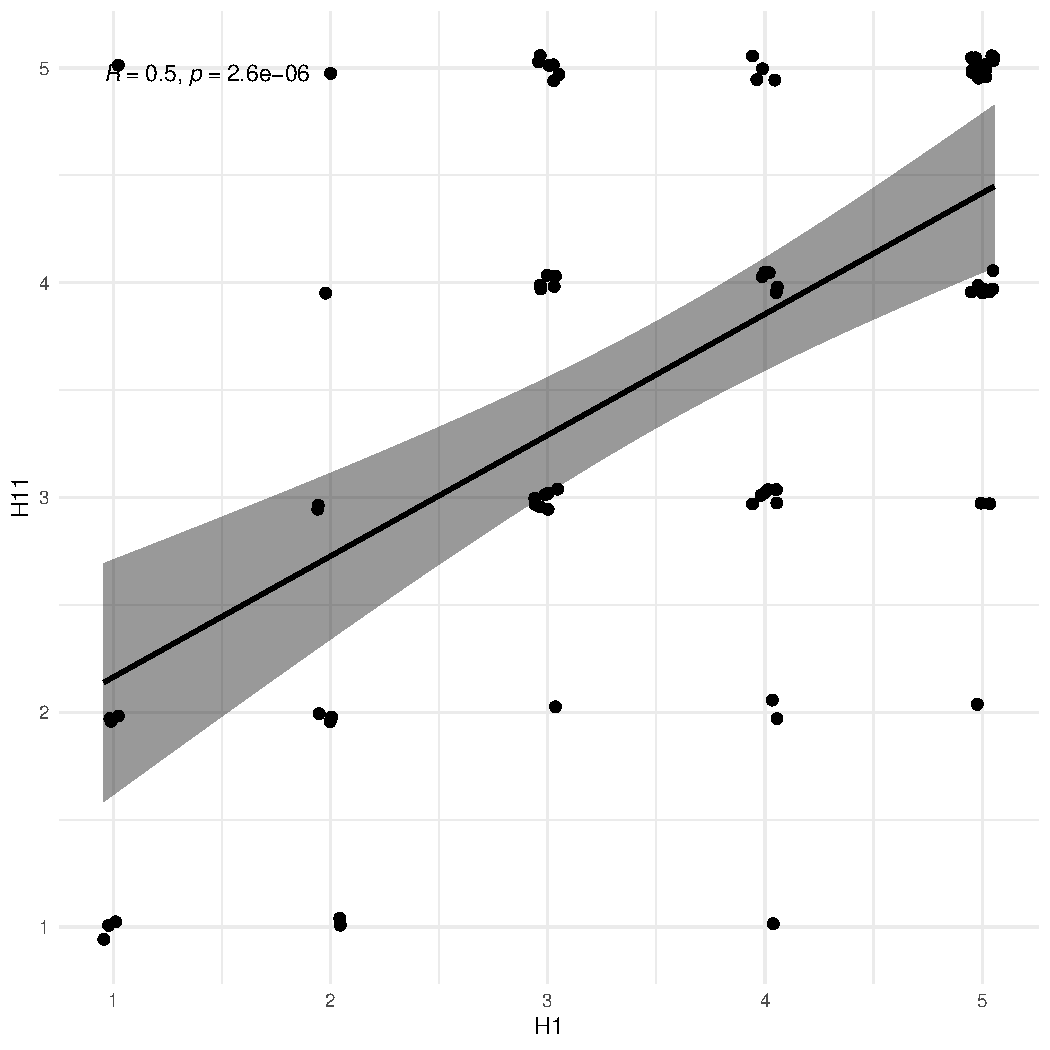
\includegraphics[width=0.65\columnwidth]{figures/plots/h1_h11.pdf}
\caption{\label{fig:h1-h11} Verwackeltes Streudiagramm - Korrelation zwischen H1 und H11}
\end{figure}

\begin{figure}[H]
\centering
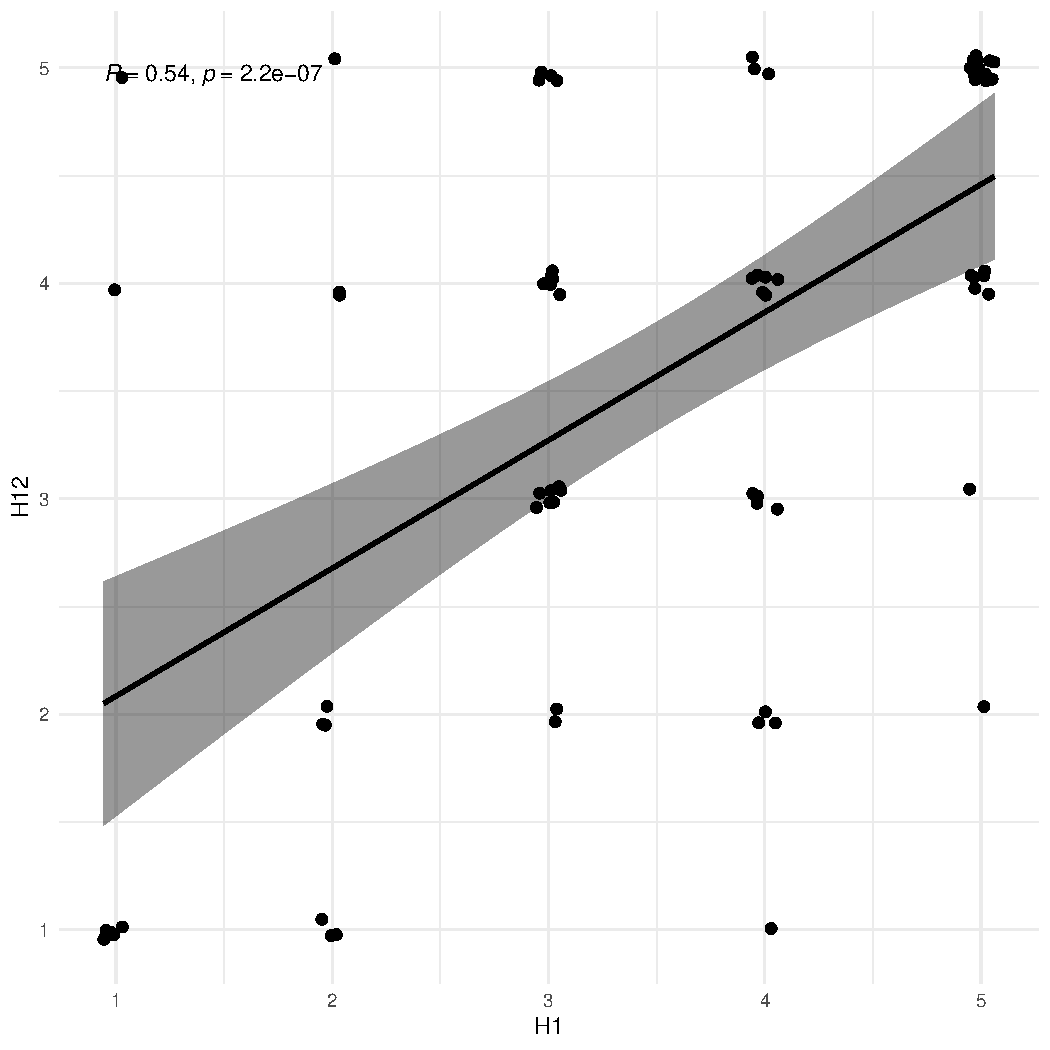
\includegraphics[width=0.65\columnwidth]{figures/plots/h1_h12.pdf}
\caption{\label{fig:h1-h12} Verwackeltes Streudiagramm - Korrelation zwischen H1 und H12}
\end{figure}

\begin{figure}[H]
\centering
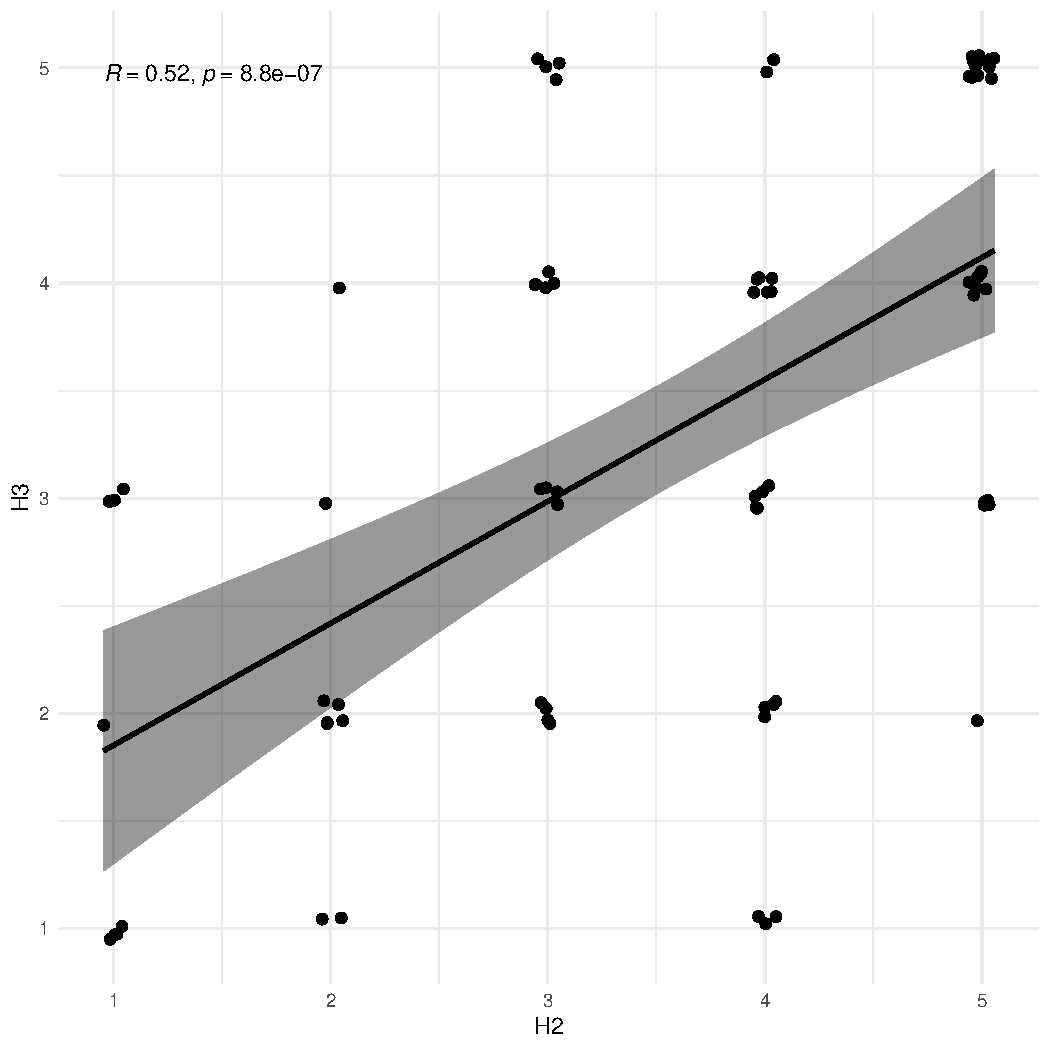
\includegraphics[width=0.65\columnwidth]{figures/plots/h2_h3.pdf}
\caption{\label{fig:h2-h3} Verwackeltes Streudiagramm - Korrelation zwischen H2 und H3}
\end{figure}


\begin{figure}[H]
\centering
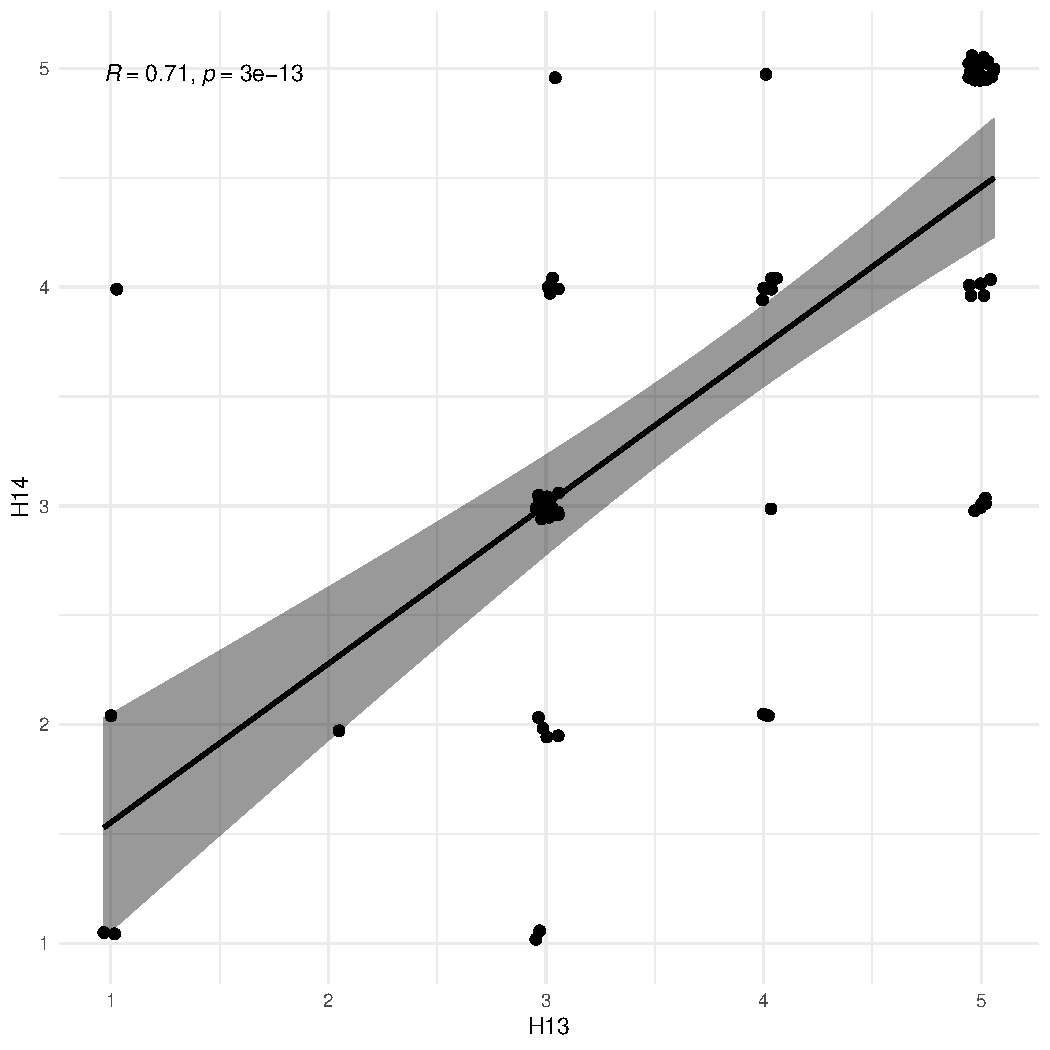
\includegraphics[width=0.65\columnwidth]{figures/plots/h13_h14.pdf}
\caption{\label{fig:h13-h14} Verwackeltes Streudiagramm - Korrelation zwischen H13 und H14}
\end{figure}